% Chapter Template

\chapter{Ensayos y Resultados} % Main chapter title

\label{Chapter4} % Change X to a consecutive number; for referencing this chapter elsewhere, use \ref{ChapterX}

%----------------------------------------------------------------------------------------
%	SECTION 1
%----------------------------------------------------------------------------------------

%\section{Pruebas funcionales del hardware}
%\label{sec:pruebasHW}

%La idea de esta sección es explicar cómo se hicieron los ensayos, qué resultados se obtuvieron y analizarlos.

\section{Validación de grafos}
	
	\subsubsection{Topología bypass}
	\subsubsection{Topología playa de maniobras}
	\subsubsection{Topología estación}
			
\section{Validación del nodo}

	La generación automática de código instancia diferentes tipos de nodos con mas o menos salidas. A la hora de realizar los ensayos se utilizó como bloque de prueba el nodo mas completo: el nodo perteneciente al tramo de vía que incluye la máquina de cambios. De esta forma se tenía la mayor cantidad de semáforos, interacciones, vecinos y comportamientos posibles.
	
	\subsection{Testbench del módulo nodo}
			
			Se generó el Algoritmo \ref{lst:test_nodo} para evaluar todas las posibles combinaciones de estados, definidas en la Tabla \ref{tabla_nodos}.
			
			
			\begin{table}[!hbt]
			\renewcommand{\arraystretch}{1.3}
			\caption{Combinaciones posibles}
			\label{tabla_nodos}
			\centering
			\begin{tabular}{ c  c  c }
			\hline
			Tramo propia & Tramo vecino & Aspecto vecino \\	
			\hline
			Ocupado & Ocupado & Rojo  \\
			Ocupado & Ocupado & Amarillo  \\
			Ocupado & Ocupado & Verde  \\	
			Ocupado & Libre & Rojo  \\
			Ocupado & Libre & Amarillo  \\
			Ocupado & Libre & Verde  \\	
			Libre & Ocupado & Rojo  \\
			Libre & Ocupado & Amarillo  \\
			Libre & Ocupado & Verde  \\	
			Libre & Libre & Rojo  \\
			Libre & Libre & Amarillo  \\
			Libre & Libre & Verde  \\	
			\end{tabular}
			\end{table}	
	
			\begin{lstlisting}[language = vhdl,caption=Testbench del módulo nodo,label={lst:test_nodo}] 
				
library ieee;
use ieee.std_logic_1164.all;
use IEEE.numeric_std.all;
--Declare the package
use work.my_package.all;

entity tb_nodo is
end tb_nodo;

architecture tb of tb_nodo is

    component nodo_1 is
		generic(
			N : natural := 21;
			N_SEM : natural := 7;
			N_MDC : natural := 1;
			N_CVS : natural := 6
		);
		port(
			Clock :  in std_logic;
			Reset :  in std_logic;
			Estado_i :  in std_logic;
			Estado_post :  in std_logic;
			Semaforo_propio_i_1 :  in sem_type;
			Semaforo_propio_o_1 :  out sem_type;
			Semaforo_cercano :  out sem_type;
			Semaforo_lejano :  out sem_type;
			Estado_o :  out std_logic
		);
    end component;

    Signal Clock : std_logic;
	Signal Reset : std_logic;
	Signal Estado_i :  std_logic;
	Signal Estado_post : std_logic;
	Signal Semaforo_propio_i_1 : sem_type;
	Signal Semaforo_propio_o_1 : sem_type;
	Signal Semaforo_cercano :  sem_type;
	Signal Semaforo_lejano :  sem_type;
	Signal Estado_o :  std_logic;

    constant TbPeriod : time := 8 ns; -- EDIT Put right period here
    signal TbClock : std_logic := '0';
    signal TbSimEnded : std_logic := '0';

begin

    dut :  nodo_1
    port map (
			  Clock      => Clock,
              Reset      => Reset,
			  Estado_i   => Estado_i,
			  Estado_post => Estado_post,
			  Semaforo_propio_i_1 => Semaforo_propio_i_1,
			  Semaforo_propio_o_1 => Semaforo_propio_o_1,
			  Semaforo_cercano => Semaforo_cercano,
			  Semaforo_lejano => Semaforo_lejano,
			  Estado_o => Estado_o
			  );

    -- Clock generation
    TbClock <= not TbClock after TbPeriod/2 when TbSimEnded /= '1' else '0';

    -- EDIT: Check that clk_i is really your main clock signal
    Clock <= TbClock;

    datos : process
    begin
        Reset <= '0';
		wait for 1 * TbPeriod;
		Reset <= '1';
		
		-- (0,0,0,0):
		Estado_i <= '0';
		Estado_post <= '0';
		Semaforo_propio_i_1.lsb <= '0';
		Semaforo_propio_i_1.msb <= '0';
		wait for 20 * TbPeriod;
		-- (0,0,0,1):
		Estado_i <= '0';
		Estado_post <= '0';
		Semaforo_propio_i_1.lsb <= '0';
		Semaforo_propio_i_1.msb <= '1';
		wait for 20 * TbPeriod;
		-- (0,0,1,1):
		Estado_i <= '0';
		Estado_post <= '0';
		Semaforo_propio_i_1.lsb <= '1';
		Semaforo_propio_i_1.msb <= '1';
		wait for 20 * TbPeriod;
		-- (0,1,0,0):
		Estado_i <= '0';
		Estado_post <= '1';
		Semaforo_propio_i_1.lsb <= '0';
		Semaforo_propio_i_1.msb <= '0';
		wait for 20 * TbPeriod;
		-- (0,1,0,1):
		Estado_i <= '0';
		Estado_post <= '1';
		Semaforo_propio_i_1.lsb <= '0';
		Semaforo_propio_i_1.msb <= '1';
		wait for 20 * TbPeriod;
		-- (0,1,1,1):
		Estado_i <= '0';
		Estado_post <= '1';
		Semaforo_propio_i_1.lsb <= '1';
		Semaforo_propio_i_1.msb <= '1';
		wait for 20 * TbPeriod;
		-- (1,0,0,0):
		Estado_i <= '1';
		Estado_post <= '0';
		Semaforo_propio_i_1.lsb <= '0';
		Semaforo_propio_i_1.msb <= '0';
		wait for 20 * TbPeriod;
		-- (1,0,0,1):
		Estado_i <= '1';
		Estado_post <= '0';
		Semaforo_propio_i_1.lsb <= '0';
		Semaforo_propio_i_1.msb <= '1';
		wait for 20 * TbPeriod;
		-- (1,0,1,1):
		Estado_i <= '1';
		Estado_post <= '0';
		Semaforo_propio_i_1.lsb <= '1';
		Semaforo_propio_i_1.msb <= '1';
		wait for 20 * TbPeriod;
		-- (1,1,0,0):
		Estado_i <= '1';
		Estado_post <= '1';
		Semaforo_propio_i_1.lsb <= '0';
		Semaforo_propio_i_1.msb <= '0';
		wait for 20 * TbPeriod;
		-- (1,1,0,1):
		Estado_i <= '1';
		Estado_post <= '1';
		Semaforo_propio_i_1.lsb <= '0';
		Semaforo_propio_i_1.msb <= '1';
		wait for 20 * TbPeriod;
		-- (1,1,1,1):
		Estado_i <= '1';
		Estado_post <= '1';
		Semaforo_propio_i_1.lsb <= '1';
		Semaforo_propio_i_1.msb <= '1';
		wait for 20 * TbPeriod;
		
        wait for 500 * TbPeriod;
	--TbSimEnded <= '1';
    end process;
	
end tb;

-- Configuration block below is required by some simulators. Usually no need to edit.

configuration cfg_tb_nodo of tb_nodo is
    for tb
    end for;
end cfg_tb_nodo;
			\end{lstlisting}
			
		\subsection{Resultados obtenidos}
			
			En la Figura \ref{fig:Test_Nodo} se muestra el resultado obtenido. Siempre que el tramo está ocupado el semáforo cambia su aspecto a rojo. Si el tramo analizado está desocupado se desprenden varios casos:
			
			\begin{itemize}
				\item Si el vecino esta ocupado: el semáforo analizado estará en aspecto rojo.
				\item Si el vecino está desocupado:
				\begin{itemize}
					\item Si el semáforo vecino está en rojo: el semáforo analizado estará en aspecto amarillo.
					\item Si el semáforo vecino está en amarillo:  el semáforo analizado estará en aspecto verde.
				\end{itemize}				 
			\end{itemize}
			
			\begin{figure}[h]
			\centering
			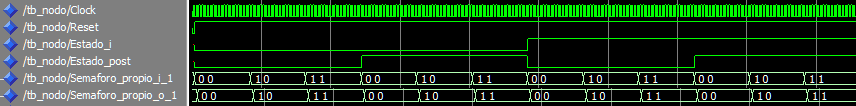
\includegraphics[scale=0.6]{./Figures/Test/Nodo}
				\caption{Simulación de un nodo}
				\label{fig:Test_Nodo}
			\end{figure}
				
			El haber validado el nodo genérico que incluye todos los posibles estados que los nodos menos complejos heredarán, se consideró que el ensayo fue un éxito.			
	
\section{Validación de la máquina de cambios}

	El módulo de la máquina de cambios tiene como función el conectar al estado anterior con el estado posterior o al estado anterior con el estado desvío según la posición del cambio de vías, como se indica en la Tabla \ref{tabla_cambios}.
	
			\begin{table}[!hbt]
			\renewcommand{\arraystretch}{1.3}
			\caption{Combinaciones posibles}
			\label{tabla_cambios}
			\centering
			\begin{tabular}{ c  c  c  c}
			\hline
			Posición del cambio & Estado anterior & Estado posterior & Estado desvío \\	
			\hline
			Normal & Ocupado & Ocupado  & Ocupado \\
			Normal & Ocupado & Ocupado  & Libre \\
			Normal & Ocupado & Libre  & Ocupado \\
			Normal & Ocupado & Libre  & Libre \\
			Normal & Libre & Ocupado  & Ocupado \\
			Normal & Libre & Ocupado  & Libre \\
			Normal & Libre & Libre  & Ocupado \\
			Normal & Libre & Libre  & Libre \\
			Inversa & Ocupado & Ocupado  & Ocupado \\
			Inversa & Ocupado & Ocupado  & Libre \\
			Inversa & Ocupado & Libre  & Ocupado \\
			Inversa & Ocupado & Libre  & Libre \\
			Inversa & Libre & Ocupado  & Ocupado \\
			Inversa & Libre & Ocupado  & Libre \\
			Inversa & Libre & Libre  & Ocupado \\
			Inversa & Libre & Libre  & Libre \\	
			\end{tabular}
			\end{table}	
	
	\subsection{Testbench del módulo de la máquina de cambios}
			
		Se generó el Algoritmo \ref{lst:test_cambios} donde se ensayan todas las combinaciones definidas en la Tabla \ref{tabla_cambios}.
			
		\begin{lstlisting}[language = vhdl,caption=Testbench del módulo de la máquina de cambios,label={lst:test_cambios}] 
				
library ieee;
use ieee.std_logic_1164.all;
use IEEE.numeric_std.all;
--Declare the package
use work.my_package.all;

entity tb_cambio is
end tb_cambio;

architecture tb of tb_cambio is

    component cambio_1 is
		generic(
			N : natural := 21;
			N_SEM : natural := 7;
			N_MDC : natural := 1;
			N_CVS : natural := 6
		);
		port(
			Clock :  in std_logic;
			Reset :  in std_logic;
			Estado_ante_i :  in std_logic;
			Estado_post_i :  in std_logic;
			Estado_desv_i :  in std_logic;
			Estado_ante_o :  out std_logic;
			Estado_post_o :  out std_logic;
			Estado_desv_o :  out std_logic;
			Cambio_i :  in std_logic;
			Cambio_o :  out std_logic
		);
    end component;

    Signal Clock : std_logic;
	Signal Reset : std_logic;
	Signal Estado_ante_i :  std_logic;
	Signal Estado_post_i : std_logic;
	Signal Estado_desv_i :  std_logic;
	Signal Estado_ante_o : std_logic;
	Signal Estado_post_o :  std_logic;
	Signal Estado_desv_o : std_logic;
	Signal Cambio_i :  std_logic;
	Signal Cambio_o : std_logic;

    constant TbPeriod : time := 8 ns; -- EDIT Put right period here
    signal TbClock : std_logic := '0';
    signal TbSimEnded : std_logic := '0';

begin

    dut :  cambio_1
    port map (
			  Clock           => Clock,
              Reset           => Reset,
			  Estado_ante_i   => Estado_ante_i,
			  Estado_post_i   => Estado_post_i,
			  Estado_desv_i   => Estado_desv_i,
			  Estado_ante_o   => Estado_ante_o,
			  Estado_post_o   => Estado_post_o,
			  Estado_desv_o   => Estado_desv_o,
			  Cambio_i        => Cambio_i,
			  Cambio_o        => Cambio_o
			  );

    -- Clock generation
    TbClock <= not TbClock after TbPeriod/2 when TbSimEnded /= '1' else '0';

    -- EDIT: Check that clk_i is really your main clock signal
    Clock <= TbClock;

    datos : process
    begin
        Reset <= '0';
		wait for 1 * TbPeriod;
		Reset <= '1';
		
		-- (0,0,0,0):
		Cambio_i <= '0';
		Estado_ante_i <= '0';
		Estado_post_i <= '0';
		Estado_desv_i <= '0';
		wait for 20 * TbPeriod;
		-- (0,0,0,1):
		Cambio_i <= '0';
		Estado_ante_i <= '0';
		Estado_post_i <= '0';
		Estado_desv_i <= '1';
		wait for 20 * TbPeriod;
		-- (0,0,1,0):
		Cambio_i <= '0';
		Estado_ante_i <= '0';
		Estado_post_i <= '1';
		Estado_desv_i <= '0';
		wait for 20 * TbPeriod;
		-- (0,0,1,1):
		Cambio_i <= '0';
		Estado_ante_i <= '0';
		Estado_post_i <= '1';
		Estado_desv_i <= '1';
		wait for 20 * TbPeriod;
		-- (0,1,0,0):
		Cambio_i <= '0';
		Estado_ante_i <= '1';
		Estado_post_i <= '0';
		Estado_desv_i <= '0';
		wait for 20 * TbPeriod;
		-- (0,1,0,1):
		Cambio_i <= '0';
		Estado_ante_i <= '1';
		Estado_post_i <= '0';
		Estado_desv_i <= '1';
		wait for 20 * TbPeriod;
		-- (0,1,1,0):
		Cambio_i <= '0';
		Estado_ante_i <= '1';
		Estado_post_i <= '1';
		Estado_desv_i <= '0';
		wait for 20 * TbPeriod;
		-- (0,1,1,1):
		Cambio_i <= '0';
		Estado_ante_i <= '1';
		Estado_post_i <= '1';
		Estado_desv_i <= '1';
		wait for 20 * TbPeriod;		
		-- (1,0,0,0):
		Cambio_i <= '1';
		Estado_ante_i <= '0';
		Estado_post_i <= '0';
		Estado_desv_i <= '0';
		wait for 20 * TbPeriod;
		-- (1,0,0,1):
		Cambio_i <= '1';
		Estado_ante_i <= '0';
		Estado_post_i <= '0';
		Estado_desv_i <= '1';
		wait for 20 * TbPeriod;
		-- (1,0,1,0):
		Cambio_i <= '1';
		Estado_ante_i <= '0';
		Estado_post_i <= '1';
		Estado_desv_i <= '0';
		wait for 20 * TbPeriod;
		-- (1,0,1,1):
		Cambio_i <= '1';
		Estado_ante_i <= '0';
		Estado_post_i <= '1';
		Estado_desv_i <= '1';
		wait for 20 * TbPeriod;
		-- (1,1,0,0):
		Cambio_i <= '1';
		Estado_ante_i <= '1';
		Estado_post_i <= '0';
		Estado_desv_i <= '0';
		wait for 20 * TbPeriod;
		-- (1,1,0,1):
		Cambio_i <= '1';
		Estado_ante_i <= '1';
		Estado_post_i <= '0';
		Estado_desv_i <= '1';
		wait for 20 * TbPeriod;
		-- (1,1,1,0):
		Cambio_i <= '1';
		Estado_ante_i <= '1';
		Estado_post_i <= '1';
		Estado_desv_i <= '0';
		wait for 20 * TbPeriod;
		-- (1,1,1,1):
		Cambio_i <= '1';
		Estado_ante_i <= '1';
		Estado_post_i <= '1';
		Estado_desv_i <= '1';
		wait for 20 * TbPeriod;
		
        wait for 500 * TbPeriod;
	--TbSimEnded <= '1';
    end process;
	
end tb;

-- Configuration block below is required by some simulators. Usually no need to edit.

configuration cfg_tb_cambio of tb_cambio is
    for tb
    end for;
end cfg_tb_cambio;
		\end{lstlisting}
			
	\subsection{Resultados obtenidos}
			
		En la Figura \ref{fig:Test_Cambios} se visualizan los resultados del ensayo. Cuando la posición de la máquina de cambios es normal entonces el estado anterior y el posterior están comunicados y cada uno puede ver tanto la ocupación como los semáforos del otro. Cuando la posición de la máquina de cambios es inversa entonces los estados vinculados son el anterior y el estado del nodo perteneciente al desvío.
		
		\begin{figure}[h]
		\centering
		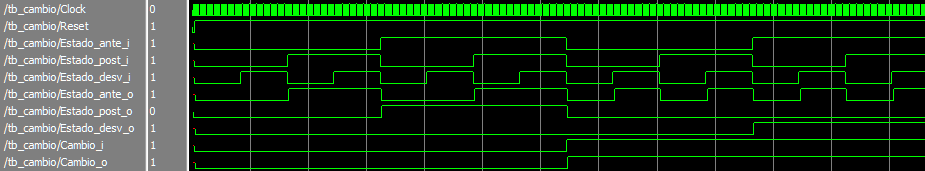
\includegraphics[scale=0.55]{./Figures/Test/Cambio}
			\caption{Simulación de la máquina de cambios}
			\label{fig:Test_Cambios}
		\end{figure}
			
		El nodo de cambios funciona de manera sincrónica y vincula correctamente los estados de los nodos involucrados. A diferencia de los bloques de nodos donde todos los nodos implementados tienen la misma cantidad de funciones que el ensayado o menor, todos los cambios tienen las mismas funcionalidades sin ninguna limitación, por lo que este ensayo unitario es suficiente para validar su correcto funcionamiento.
				
\section{Validación de la UART}

	En el diseño del sistema se contempló utilizar uno de los switches de la placa de desarrollo para poder puentear todo el enclavamiento y probar fácilmente el funcionamiento de la UART sin el efecto del enclavamiento. En esta sección se realizó el ensayo con el switch en la posición en la cual la salida recibe el mensaje de la entrada directamente, sin pasar por ningun otro bloque.

	\subsection{Testbench del módulo UART}
			
		Se generó el Algoritmo \ref{lst:test_uart} en el cual se inyecta la entrada de la UART directamente a la salida de la UART, teniendo una prueba echo. Todos los mensajes ingresados, siempre que sean válidos, pasarán a la salida para ser publicados en la terminal desde donde se originaron.
			
		\begin{lstlisting}[language = vhdl,caption=Testbench del módulo UART,label={lst:test_uart}] 
library ieee;
use ieee.std_logic_1164.all;

entity tb_sistema is
end tb_sistema;

architecture tb of tb_sistema is

    component sistema
       port(
		Clock: in std_logic;
        	Reset: in std_logic;
			r_data: in std_logic_vector(8-1 downto 0);
			r_disponible : in std_logic;
			leer : out std_logic;
			escribir : out std_logic;
			switch1 : in std_logic;
			switch2 : in std_logic;
			reset_uart : out std_logic;
			N : in integer;
			leds : out std_logic_vector(4-1 downto 0);
			led_rgb_1  : out std_logic_vector(3-1 downto 0);
			led_rgb_2  : out std_logic_vector(3-1 downto 0);
			w_data: out std_logic_vector(8-1 downto 0)
		);
    end component;


    signal Clock     : std_logic;
    signal Reset     : std_logic;
    signal r_data    : std_logic_vector (8-1 downto 0);
    signal r_disponible : std_logic;
    signal leer : std_logic;
    signal escribir : std_logic;
    signal switch1    : std_logic;
    signal switch2   : std_logic;
    signal reset_uart : std_logic;
    signal N : integer;
    signal leds      : std_logic_vector(4-1 downto 0);
    signal led_rgb_1 : std_logic_vector (3-1 downto 0);
    signal led_rgb_2 : std_logic_vector (3-1 downto 0);

    signal w_data    : std_logic_vector (8-1 downto 0);

    constant TbPeriod : time := 8 ns; -- EDIT Put right period here
    signal TbClock : std_logic := '0';
    signal TbSimEnded : std_logic := '0';

    constant periodo : integer := 100;

	 -- Low-level byte-write
  	procedure Enviar_char (
    		data       : in  std_logic_vector(8-1 downto 0);
    		signal r_data : out std_logic_vector(8-1 downto 0);
		signal r_disponible : out std_logic) is
  	begin

   		r_disponible <= '0';
		wait for TbPeriod;
        r_data <= data;
		wait for TbPeriod;
		r_disponible <= '1';
		wait for TbPeriod;
		r_disponible <= '0';

  	end Enviar_char;

begin

    dut : sistema
    port map (Clock      => Clock,
              Reset      => Reset,
              r_data     => r_data,
	          r_disponible => r_disponible,
	          leer       => leer,
 	     	  escribir   => escribir,
	      	  switch1    => switch1,
	     	  switch2    => switch2,
	     	  reset_uart => reset_uart,
   	     	  N          => N,
	     	  leds 	 => leds,
              led_rgb_1  => led_rgb_1,
              led_rgb_2  => led_rgb_2,
              w_data     => w_data);

    -- Clock generation
    TbClock <= not TbClock after TbPeriod/2 when TbSimEnded /= '1' else '0';

    -- EDIT: Check that clk_i is really your main clock signal
    Clock <= TbClock;

    stimuli : process
    begin
        -- EDIT Adapt initialization as needed
        --r_data <= (others => '0');

        -- Reset generation
        -- EDIT: Check that rst_i is really your reset signal
		switch1 <= '1';
		switch2 <= '0';
        Reset <= '1';
        wait for 100 ns;
        Reset <= '0';
		switch1 <= '1';
		switch2 <= '0';
        wait for 250000 * TbPeriod;

        -- Stop the clock and hence terminate the simulation
        TbSimEnded <= '1';
        wait;
    end process;

    datos : process
    begin
        
	r_data <= "00000000";
	r_disponible <= '0';

	wait for 100 ns;

	-- 21 - 21 - todos 1
	N <= 23; 	
	Enviar_char("00111100",r_data,r_disponible); -- < 	
	Enviar_char("00110001",r_data,r_disponible); -- 1 	
	Enviar_char("00110001",r_data,r_disponible); -- 1
 	Enviar_char("00110001",r_data,r_disponible); -- 1 	
	Enviar_char("00110001",r_data,r_disponible); -- 1
	Enviar_char("00110001",r_data,r_disponible); -- 1 	
	Enviar_char("00110001",r_data,r_disponible); -- 1
	Enviar_char("00110001",r_data,r_disponible); -- 1 	
	Enviar_char("00110001",r_data,r_disponible); -- 1
	Enviar_char("00110001",r_data,r_disponible); -- 1 	
	Enviar_char("00110001",r_data,r_disponible); -- 1
	Enviar_char("00110001",r_data,r_disponible); -- 1 	
	Enviar_char("00110001",r_data,r_disponible); -- 1
	Enviar_char("00110001",r_data,r_disponible); -- 1 	
	Enviar_char("00110001",r_data,r_disponible); -- 1
	Enviar_char("00110001",r_data,r_disponible); -- 1 	
	Enviar_char("00110001",r_data,r_disponible); -- 1
	Enviar_char("00110001",r_data,r_disponible); -- 1 	
	Enviar_char("00110001",r_data,r_disponible); -- 1
	Enviar_char("00110001",r_data,r_disponible); -- 1 	
	Enviar_char("00110001",r_data,r_disponible); -- 1
	Enviar_char("00110001",r_data,r_disponible); -- 1 	
	Enviar_char("00111110",r_data,r_disponible); -- >

	wait for periodo * TbPeriod;

	-- 21 - 1
	N <= 23; 	
	Enviar_char("00111100",r_data,r_disponible); -- < 	
	Enviar_char("00110000",r_data,r_disponible); -- 0 	
	Enviar_char("00110000",r_data,r_disponible); -- 0
 	Enviar_char("00110000",r_data,r_disponible); -- 0 	
	Enviar_char("00110000",r_data,r_disponible); -- 0
	Enviar_char("00110000",r_data,r_disponible); -- 0 	
	Enviar_char("00110000",r_data,r_disponible); -- 0
	Enviar_char("00110000",r_data,r_disponible); -- 0 	
	Enviar_char("00110000",r_data,r_disponible); -- 0
	Enviar_char("00110000",r_data,r_disponible); -- 0 	
	Enviar_char("00110000",r_data,r_disponible); -- 0
	Enviar_char("00110000",r_data,r_disponible); -- 0 	
	Enviar_char("00110000",r_data,r_disponible); -- 0
	Enviar_char("00110000",r_data,r_disponible); -- 0 	
	Enviar_char("00110000",r_data,r_disponible); -- 0
	Enviar_char("00110000",r_data,r_disponible); -- 0 	
	Enviar_char("00110000",r_data,r_disponible); -- 0
	Enviar_char("00110000",r_data,r_disponible); -- 0 	
	Enviar_char("00110000",r_data,r_disponible); -- 0
	Enviar_char("00110000",r_data,r_disponible); -- 0 	
	Enviar_char("00110000",r_data,r_disponible); -- 0
	Enviar_char("00110001",r_data,r_disponible); -- 1 	
	Enviar_char("00111110",r_data,r_disponible); -- >

	wait for periodo * TbPeriod;

	-- 21 - 2
	N <= 23; 	
	Enviar_char("00111100",r_data,r_disponible); -- < 	
	Enviar_char("00110000",r_data,r_disponible); -- 0 	
	Enviar_char("00110000",r_data,r_disponible); -- 0
 	Enviar_char("00110000",r_data,r_disponible); -- 0 	
	Enviar_char("00110000",r_data,r_disponible); -- 0
	Enviar_char("00110000",r_data,r_disponible); -- 0 	
	Enviar_char("00110000",r_data,r_disponible); -- 0
	Enviar_char("00110000",r_data,r_disponible); -- 0 	
	Enviar_char("00110000",r_data,r_disponible); -- 0
	Enviar_char("00110000",r_data,r_disponible); -- 0 	
	Enviar_char("00110000",r_data,r_disponible); -- 0
	Enviar_char("00110000",r_data,r_disponible); -- 0 	
	Enviar_char("00110000",r_data,r_disponible); -- 0
	Enviar_char("00110000",r_data,r_disponible); -- 0 	
	Enviar_char("00110000",r_data,r_disponible); -- 0
	Enviar_char("00110000",r_data,r_disponible); -- 0 	
	Enviar_char("00110000",r_data,r_disponible); -- 0
	Enviar_char("00110000",r_data,r_disponible); -- 0 	
	Enviar_char("00110000",r_data,r_disponible); -- 0
	Enviar_char("00110000",r_data,r_disponible); -- 0 	
	Enviar_char("00110001",r_data,r_disponible); -- 1
	Enviar_char("00110000",r_data,r_disponible); -- 0 	
	Enviar_char("00111110",r_data,r_disponible); -- >

	wait for periodo * TbPeriod;
	
	-- Moviendo el "1" en todas las posiciones --

	-- Borrado para la memoria para resumir --
	
	-- Moviendo el "1" en todas las posiciones --
	
	-- 21 - 20
	N <= 23; 	
	Enviar_char("00111100",r_data,r_disponible); -- < 	
	Enviar_char("00110000",r_data,r_disponible); -- 0 	
	Enviar_char("00110001",r_data,r_disponible); -- 1
 	Enviar_char("00110000",r_data,r_disponible); -- 0 	
	Enviar_char("00110000",r_data,r_disponible); -- 0
	Enviar_char("00110000",r_data,r_disponible); -- 0 	
	Enviar_char("00110000",r_data,r_disponible); -- 0
	Enviar_char("00110000",r_data,r_disponible); -- 0 	
	Enviar_char("00110000",r_data,r_disponible); -- 0
	Enviar_char("00110000",r_data,r_disponible); -- 0 	
	Enviar_char("00110000",r_data,r_disponible); -- 0
	Enviar_char("00110000",r_data,r_disponible); -- 0 	
	Enviar_char("00110000",r_data,r_disponible); -- 0
	Enviar_char("00110000",r_data,r_disponible); -- 0 	
	Enviar_char("00110000",r_data,r_disponible); -- 0
	Enviar_char("00110000",r_data,r_disponible); -- 0 	
	Enviar_char("00110000",r_data,r_disponible); -- 0
	Enviar_char("00110000",r_data,r_disponible); -- 0 	
	Enviar_char("00110000",r_data,r_disponible); -- 0
	Enviar_char("00110000",r_data,r_disponible); -- 0 	
	Enviar_char("00110000",r_data,r_disponible); -- 0
	Enviar_char("00110000",r_data,r_disponible); -- 0 	
	Enviar_char("00111110",r_data,r_disponible); -- >

	wait for periodo * TbPeriod;

	-- 21 - 21
	N <= 23; 	
	Enviar_char("00111100",r_data,r_disponible); -- < 	
	Enviar_char("00110001",r_data,r_disponible); -- 1 	
	Enviar_char("00110000",r_data,r_disponible); -- 0
 	Enviar_char("00110000",r_data,r_disponible); -- 0 	
	Enviar_char("00110000",r_data,r_disponible); -- 0
	Enviar_char("00110000",r_data,r_disponible); -- 0 	
	Enviar_char("00110000",r_data,r_disponible); -- 0
	Enviar_char("00110000",r_data,r_disponible); -- 0 	
	Enviar_char("00110000",r_data,r_disponible); -- 0
	Enviar_char("00110000",r_data,r_disponible); -- 0 	
	Enviar_char("00110000",r_data,r_disponible); -- 0
	Enviar_char("00110000",r_data,r_disponible); -- 0 	
	Enviar_char("00110000",r_data,r_disponible); -- 0
	Enviar_char("00110000",r_data,r_disponible); -- 0 	
	Enviar_char("00110000",r_data,r_disponible); -- 0
	Enviar_char("00110000",r_data,r_disponible); -- 0 	
	Enviar_char("00110000",r_data,r_disponible); -- 0
	Enviar_char("00110000",r_data,r_disponible); -- 0 	
	Enviar_char("00110000",r_data,r_disponible); -- 0
	Enviar_char("00110000",r_data,r_disponible); -- 0 	
	Enviar_char("00110000",r_data,r_disponible); -- 0
	Enviar_char("00110000",r_data,r_disponible); -- 0 	
	Enviar_char("00111110",r_data,r_disponible); -- >

	wait for periodo * TbPeriod;

	-- 22
	N <= 24; 	
	Enviar_char("00111100",r_data,r_disponible); -- < 	
	Enviar_char("00110001",r_data,r_disponible); -- 1 	
	Enviar_char("00110000",r_data,r_disponible); -- 0
 	Enviar_char("00110001",r_data,r_disponible); -- 1 	
	Enviar_char("00110000",r_data,r_disponible); -- 0
	Enviar_char("00110001",r_data,r_disponible); -- 1 	
	Enviar_char("00110000",r_data,r_disponible); -- 0
	Enviar_char("00110001",r_data,r_disponible); -- 1 	
	Enviar_char("00110000",r_data,r_disponible); -- 0
	Enviar_char("00110001",r_data,r_disponible); -- 1 	
	Enviar_char("00110000",r_data,r_disponible); -- 0
	Enviar_char("00110001",r_data,r_disponible); -- 1 	
	Enviar_char("00110000",r_data,r_disponible); -- 0
	Enviar_char("00110001",r_data,r_disponible); -- 1 	
	Enviar_char("00110000",r_data,r_disponible); -- 0
	Enviar_char("00110001",r_data,r_disponible); -- 1 	
	Enviar_char("00110000",r_data,r_disponible); -- 0
	Enviar_char("00110001",r_data,r_disponible); -- 1 	
	Enviar_char("00110000",r_data,r_disponible); -- 0
	Enviar_char("00110001",r_data,r_disponible); -- 1 	
	Enviar_char("00110000",r_data,r_disponible); -- 0
	Enviar_char("00110001",r_data,r_disponible); -- 1 
	Enviar_char("00110000",r_data,r_disponible); -- 0	
	Enviar_char("00111110",r_data,r_disponible); -- >
	
        wait for periodo * TbPeriod;
	TbSimEnded <= '1';
    end process;
	
end tb;

		\end{lstlisting}
			
	\subsection{Resultados obtenidos}
				
		En la Figura \ref{fig:TEST_Uart} se presentan los datos del ensayo. Se puede ver que las tramas inyectadas son presentadas idénticamente en la salida, con un pequeño delay temporal. Además de poder apreciar el tren de pulsos que envía la UART de un extremo al otro del módulo, primero para indicar la lectura de la FIFO de recepción y luego para indicar la escritura de la FIFO de transmisión.
		
		\begin{figure}[h]
		\centering
		%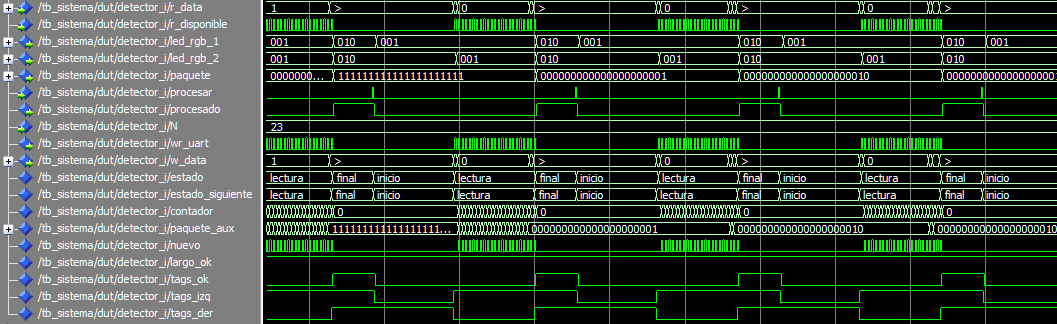
\includegraphics[scale=0.5]{./Figures/Test/Detector}
			\caption{Simulación de la UART}
			\label{fig:Test_UART}
		\end{figure}
			
		Solo después de superado este ensayo se pudo avanzar con la inclusión de los demás módulos. No tenía ningún sentido implementar sistemas complejos sin la certeza de que la transmisión y recepción de datos de la computadora a la plataforma era fiable. Este proceso de desarrollo requirió varias iteraciones por la dificultad que implicó depurar cada uno de los elementos involucrados.
	
\section{Validación del detector}

	\subsection{Testbench del módulo detector}
			
		Se generó el Algoritmo \ref{lst:test_detector} para ...
		
			
		\begin{lstlisting}[language = vhdl,caption=Testbench del módulo detector,label={lst:test_detector}] 
				
			library ieee;
use ieee.std_logic_1164.all;

entity tb_detector is
end tb_detector;

architecture tb of tb_detector is

    component detector
        port(
		clk_i: in std_logic;
       		rst_i: in std_logic;
		r_data: in std_logic_vector(8-1 downto 0);
		r_disponible : in std_logic;
		led_rgb_1  : out std_logic_vector(3-1 downto 0);
		led_rgb_2  : out std_logic_vector(3-1 downto 0);
		paquete: out std_logic_vector(21-1 downto 0);
		procesar : in std_logic;
		procesado : out std_logic;
		N : in integer;
		N_1 : out integer;
		N_2 : out integer;
		wr_uart : out std_logic;
		w_data: out std_logic_vector(8-1 downto 0)
	);
    end component;

    signal clk_i     : std_logic;
    signal rst_i     : std_logic;
    signal r_data    : std_logic_vector (8-1 downto 0);
    signal r_disponible      : std_logic;
    signal led_rgb_1 : std_logic_vector (3-1 downto 0);
    signal led_rgb_2 : std_logic_vector (3-1 downto 0);
    signal paquete   : std_logic_vector (21-1 downto 0); 
    signal procesar : std_logic;
    signal procesado : std_logic;
    signal N,N_1,N_2 : integer;
    signal wr_uart : std_logic;
    signal w_data    : std_logic_vector (8-1 downto 0);

    constant TbPeriod : time := 8 ns; -- EDIT Put right period here
    signal TbClock : std_logic := '0';
    signal TbSimEnded : std_logic := '0';

	 -- Low-level byte-write
  	procedure Enviar_char (
    		data       : in  std_logic_vector(8-1 downto 0);
    		signal r_data : out std_logic_vector(8-1 downto 0);
		signal r_disponible : out std_logic) is
  	begin

   		r_disponible <= '0';
		wait for TbPeriod;
        	r_data <= data;
		wait for TbPeriod;
		r_disponible <= '1';
		wait for TbPeriod;
		r_disponible <= '0';

  	end Enviar_char;

begin

    dut : detector
    port map (clk_i      => clk_i,
              rst_i      => rst_i,
              r_data     => r_data,
	      r_disponible => r_disponible,
              led_rgb_1  => led_rgb_1,
              led_rgb_2  => led_rgb_2,
              paquete    => paquete,
	      procesar   => procesar,
      	      procesado  => procesado,
	      N 	 => N,
              N_1        => N_1,
 	      N_2 	 => N_2,
	      wr_uart    => wr_uart,
              w_data     => w_data);

    -- Clock generation
    TbClock <= not TbClock after TbPeriod/2 when TbSimEnded /= '1' else '0';

    -- EDIT: Check that clk_i is really your main clock signal
    clk_i <= TbClock;

    stimuli : process
    begin
        -- EDIT Adapt initialization as needed
        --r_data <= (others => '0');

        -- Reset generation
        -- EDIT: Check that rst_i is really your reset signal
        rst_i <= '1';
        wait for 100 ns;
        rst_i <= '0';

	
        wait for 1000 * TbPeriod;

        -- Stop the clock and hence terminate the simulation
        TbSimEnded <= '1';
        wait;
    end process;

    datos : process
    begin
        
	r_data <= "00000000";
	r_disponible <= '0';

	wait for 100 ns;

	-- 21
	N <= 23; 	
	Enviar_char("00111100",r_data,r_disponible); -- < 	
	Enviar_char("00110001",r_data,r_disponible); -- 1 	
	Enviar_char("00110001",r_data,r_disponible); -- 1
 	Enviar_char("00110001",r_data,r_disponible); -- 1 	
	Enviar_char("00110000",r_data,r_disponible); -- 0
	Enviar_char("00110001",r_data,r_disponible); -- 1 	
	Enviar_char("00110000",r_data,r_disponible); -- 0
	Enviar_char("00110001",r_data,r_disponible); -- 1 	
	Enviar_char("00110000",r_data,r_disponible); -- 0
	Enviar_char("00110001",r_data,r_disponible); -- 1 	
	Enviar_char("00110000",r_data,r_disponible); -- 0
	Enviar_char("00110001",r_data,r_disponible); -- 1 	
	Enviar_char("00110000",r_data,r_disponible); -- 0
	Enviar_char("00110001",r_data,r_disponible); -- 1 	
	Enviar_char("00110000",r_data,r_disponible); -- 0
	Enviar_char("00110001",r_data,r_disponible); -- 1 	
	Enviar_char("00110000",r_data,r_disponible); -- 0
	Enviar_char("00110001",r_data,r_disponible); -- 1 	
	Enviar_char("00110000",r_data,r_disponible); -- 0
	Enviar_char("00110000",r_data,r_disponible); -- 0 	
	Enviar_char("00110001",r_data,r_disponible); -- 1
	Enviar_char("00110001",r_data,r_disponible); -- 1 	
	Enviar_char("00111110",r_data,r_disponible); -- >

	wait for 100 * TbPeriod;

	-- 21
	N <= 23; 	
	Enviar_char("00111100",r_data,r_disponible); -- < 	
	Enviar_char("00110001",r_data,r_disponible); -- 1 	
	Enviar_char("00110001",r_data,r_disponible); -- 1
 	Enviar_char("00110001",r_data,r_disponible); -- 1 	
	Enviar_char("00110000",r_data,r_disponible); -- 0
	Enviar_char("00110001",r_data,r_disponible); -- 1 	
	Enviar_char("00110000",r_data,r_disponible); -- 0
	Enviar_char("00110001",r_data,r_disponible); -- 1 	
	Enviar_char("00110000",r_data,r_disponible); -- 0
	Enviar_char("00110001",r_data,r_disponible); -- 1 	
	Enviar_char("00110000",r_data,r_disponible); -- 0
	Enviar_char("00110001",r_data,r_disponible); -- 1 	
	Enviar_char("00110000",r_data,r_disponible); -- 0
	Enviar_char("00110001",r_data,r_disponible); -- 1 	
	Enviar_char("00110000",r_data,r_disponible); -- 0
	Enviar_char("00110001",r_data,r_disponible); -- 1 	
	Enviar_char("00110000",r_data,r_disponible); -- 0
	Enviar_char("00110001",r_data,r_disponible); -- 1 	
	Enviar_char("00110000",r_data,r_disponible); -- 0
	Enviar_char("00110000",r_data,r_disponible); -- 0 	
	Enviar_char("00110001",r_data,r_disponible); -- 1
	Enviar_char("00110001",r_data,r_disponible); -- 1 	
	Enviar_char("00111110",r_data,r_disponible); -- >

	wait for 100 * TbPeriod;

	-- 22
	N <= 24; 	
	Enviar_char("00111100",r_data,r_disponible); -- < 	
	Enviar_char("00110001",r_data,r_disponible); -- 1 	
	Enviar_char("00110000",r_data,r_disponible); -- 0
 	Enviar_char("00110001",r_data,r_disponible); -- 1 	
	Enviar_char("00110000",r_data,r_disponible); -- 0
	Enviar_char("00110001",r_data,r_disponible); -- 1 	
	Enviar_char("00110000",r_data,r_disponible); -- 0
	Enviar_char("00110001",r_data,r_disponible); -- 1 	
	Enviar_char("00110000",r_data,r_disponible); -- 0
	Enviar_char("00110001",r_data,r_disponible); -- 1 	
	Enviar_char("00110000",r_data,r_disponible); -- 0
	Enviar_char("00110001",r_data,r_disponible); -- 1 	
	Enviar_char("00110000",r_data,r_disponible); -- 0
	Enviar_char("00110001",r_data,r_disponible); -- 1 	
	Enviar_char("00110000",r_data,r_disponible); -- 0
	Enviar_char("00110001",r_data,r_disponible); -- 1 	
	Enviar_char("00110000",r_data,r_disponible); -- 0
	Enviar_char("00110001",r_data,r_disponible); -- 1 	
	Enviar_char("00110000",r_data,r_disponible); -- 0
	Enviar_char("00110001",r_data,r_disponible); -- 1 	
	Enviar_char("00110000",r_data,r_disponible); -- 0
	Enviar_char("00110001",r_data,r_disponible); -- 1 
	Enviar_char("00110000",r_data,r_disponible); -- 0	
	Enviar_char("00111110",r_data,r_disponible); -- >
	
	wait for 100 * TbPeriod;

	-- 21
	N <= 23; 	
	Enviar_char("00111100",r_data,r_disponible); -- < 	
	Enviar_char("00110001",r_data,r_disponible); -- 1 	
	Enviar_char("00110001",r_data,r_disponible); -- 1
 	Enviar_char("00110001",r_data,r_disponible); -- 1 	
	Enviar_char("00110000",r_data,r_disponible); -- 0
	Enviar_char("00110001",r_data,r_disponible); -- 1 	
	Enviar_char("00110000",r_data,r_disponible); -- 0
	Enviar_char("00110001",r_data,r_disponible); -- 1 	
	Enviar_char("00110000",r_data,r_disponible); -- 0
	Enviar_char("00110001",r_data,r_disponible); -- 1 	
	Enviar_char("00110000",r_data,r_disponible); -- 0
	Enviar_char("00110001",r_data,r_disponible); -- 1 	
	Enviar_char("00110000",r_data,r_disponible); -- 0
	Enviar_char("00110001",r_data,r_disponible); -- 1 	
	Enviar_char("00110000",r_data,r_disponible); -- 0
	Enviar_char("00110001",r_data,r_disponible); -- 1 	
	Enviar_char("00110000",r_data,r_disponible); -- 0
	Enviar_char("00110001",r_data,r_disponible); -- 1 	
	Enviar_char("00110000",r_data,r_disponible); -- 0
	Enviar_char("00110000",r_data,r_disponible); -- 0 	
	Enviar_char("00110001",r_data,r_disponible); -- 1
	Enviar_char("00110001",r_data,r_disponible); -- 1 	
	Enviar_char("00111110",r_data,r_disponible); -- >


        wait for 100 * TbPeriod;
	TbSimEnded <= '1';
    end process;
	
end tb;
		\end{lstlisting}
			
	\subsection{Resultados obtenidos}
				
		Figura \ref{fig:Test_Detector} ...
		
		\begin{figure}[h]
		\centering
		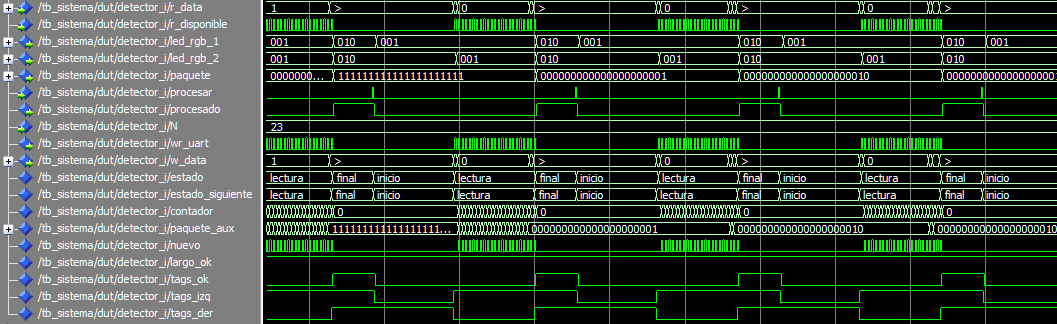
\includegraphics[scale=0.5]{./Figures/Test/Detector}
			\caption{Simulación del detector}
			\label{fig:Test_Detector}
		\end{figure}

\section{Validación del enclavamiento}	

	\subsection{Testbench del módulo enclavamiento}
			
		Se generó el Algoritmo \ref{lst:test_enclavamiento} para ...
		
			
		\begin{lstlisting}[language = vhdl,caption=Testbench del módulo enclavamiento,label={lst:test_separador}] 
				
			library ieee;
use ieee.std_logic_1164.all;

entity tb_sistema is
end tb_sistema;

architecture tb of tb_sistema is

    component sistema
       port(
		Clock: in std_logic;
        	Reset: in std_logic;
		r_data: in std_logic_vector(8-1 downto 0);
		r_disponible : in std_logic;
		leer : out std_logic;
		escribir : out std_logic;
		switch1 : in std_logic;
		switch2 : in std_logic;
		reset_uart : out std_logic;
		N : in integer;
		--leds : out std_logic_vector(2-1 downto 0);
		leds : out std_logic_vector(4-1 downto 0);
		led_rgb_1  : out std_logic_vector(3-1 downto 0);
		led_rgb_2  : out std_logic_vector(3-1 downto 0);
		w_data: out std_logic_vector(8-1 downto 0)
	);
    end component;


    signal Clock     : std_logic;
    signal Reset     : std_logic;
    signal r_data    : std_logic_vector (8-1 downto 0);
    signal r_disponible : std_logic;
    signal leer : std_logic;
    signal escribir : std_logic;
    signal switch1    : std_logic;
    signal switch2   : std_logic;
    signal reset_uart : std_logic;
    signal N : integer;
    signal leds      : std_logic_vector(4-1 downto 0);
    signal led_rgb_1 : std_logic_vector (3-1 downto 0);
    signal led_rgb_2 : std_logic_vector (3-1 downto 0);

    signal w_data    : std_logic_vector (8-1 downto 0);

    constant TbPeriod : time := 8 ns; -- EDIT Put right period here
    signal TbClock : std_logic := '0';
    signal TbSimEnded : std_logic := '0';

    constant periodo : integer := 100;

	 -- Low-level byte-write
  	procedure Enviar_char (
    		data       : in  std_logic_vector(8-1 downto 0);
    		signal r_data : out std_logic_vector(8-1 downto 0);
		signal r_disponible : out std_logic) is
  	begin

   		r_disponible <= '0';
		wait for TbPeriod;
        	r_data <= data;
		wait for TbPeriod;
		r_disponible <= '1';
		wait for TbPeriod;
		r_disponible <= '0';

  	end Enviar_char;

begin

    dut : sistema
    port map (Clock      => Clock,
              Reset      => Reset,
              r_data     => r_data,
	      r_disponible => r_disponible,
	      leer       => leer,
 	      escribir   => escribir,
	      switch1    => switch1,
	      switch2    => switch2,
	      reset_uart => reset_uart,
   	      N          => N,
	      leds 	 => leds,
              led_rgb_1  => led_rgb_1,
              led_rgb_2  => led_rgb_2,
              w_data     => w_data);

    -- Clock generation
    TbClock <= not TbClock after TbPeriod/2 when TbSimEnded /= '1' else '0';

    -- EDIT: Check that clk_i is really your main clock signal
    Clock <= TbClock;

    stimuli : process
    begin
        -- EDIT Adapt initialization as needed
        --r_data <= (others => '0');

        -- Reset generation
        -- EDIT: Check that rst_i is really your reset signal
	switch1 <= '1';
	switch2 <= '1';
        Reset <= '1';
        wait for 100 ns;
        Reset <= '0';
	switch1 <= '1';
	switch2 <= '1';
        wait for 250000 * TbPeriod;

        -- Stop the clock and hence terminate the simulation
        TbSimEnded <= '1';
        wait;
    end process;

    datos : process
    begin
        
	r_data <= "00000000";
	r_disponible <= '0';

	wait for 100 ns;

	-- 21 - 21 - todos 1
	N <= 23; 	
	Enviar_char("00111100",r_data,r_disponible); -- < 	
	Enviar_char("00110001",r_data,r_disponible); -- 1 	
	Enviar_char("00110001",r_data,r_disponible); -- 1
 	Enviar_char("00110001",r_data,r_disponible); -- 1 	
	Enviar_char("00110001",r_data,r_disponible); -- 1
	Enviar_char("00110001",r_data,r_disponible); -- 1 	
	Enviar_char("00110001",r_data,r_disponible); -- 1
	Enviar_char("00110001",r_data,r_disponible); -- 1 	
	Enviar_char("00110001",r_data,r_disponible); -- 1
	Enviar_char("00110001",r_data,r_disponible); -- 1 	
	Enviar_char("00110001",r_data,r_disponible); -- 1
	Enviar_char("00110001",r_data,r_disponible); -- 1 	
	Enviar_char("00110001",r_data,r_disponible); -- 1
	Enviar_char("00110001",r_data,r_disponible); -- 1 	
	Enviar_char("00110001",r_data,r_disponible); -- 1
	Enviar_char("00110001",r_data,r_disponible); -- 1 	
	Enviar_char("00110001",r_data,r_disponible); -- 1
	Enviar_char("00110001",r_data,r_disponible); -- 1 	
	Enviar_char("00110001",r_data,r_disponible); -- 1
	Enviar_char("00110001",r_data,r_disponible); -- 1 	
	Enviar_char("00110001",r_data,r_disponible); -- 1
	Enviar_char("00110001",r_data,r_disponible); -- 1 	
	Enviar_char("00111110",r_data,r_disponible); -- >

	wait for periodo * TbPeriod;

	-- 21 - 1
	N <= 23; 	
	Enviar_char("00111100",r_data,r_disponible); -- < 	
	Enviar_char("00110000",r_data,r_disponible); -- 0 	
	Enviar_char("00110000",r_data,r_disponible); -- 0
 	Enviar_char("00110000",r_data,r_disponible); -- 0 	
	Enviar_char("00110000",r_data,r_disponible); -- 0
	Enviar_char("00110000",r_data,r_disponible); -- 0 	
	Enviar_char("00110000",r_data,r_disponible); -- 0
	Enviar_char("00110000",r_data,r_disponible); -- 0 	
	Enviar_char("00110000",r_data,r_disponible); -- 0
	Enviar_char("00110000",r_data,r_disponible); -- 0 	
	Enviar_char("00110000",r_data,r_disponible); -- 0
	Enviar_char("00110000",r_data,r_disponible); -- 0 	
	Enviar_char("00110000",r_data,r_disponible); -- 0
	Enviar_char("00110000",r_data,r_disponible); -- 0 	
	Enviar_char("00110000",r_data,r_disponible); -- 0
	Enviar_char("00110000",r_data,r_disponible); -- 0 	
	Enviar_char("00110000",r_data,r_disponible); -- 0
	Enviar_char("00110000",r_data,r_disponible); -- 0 	
	Enviar_char("00110000",r_data,r_disponible); -- 0
	Enviar_char("00110000",r_data,r_disponible); -- 0 	
	Enviar_char("00110000",r_data,r_disponible); -- 0
	Enviar_char("00110001",r_data,r_disponible); -- 1 	
	Enviar_char("00111110",r_data,r_disponible); -- >

	wait for periodo * TbPeriod;

	-- 21 - 2
	N <= 23; 	
	Enviar_char("00111100",r_data,r_disponible); -- < 	
	Enviar_char("00110000",r_data,r_disponible); -- 0 	
	Enviar_char("00110000",r_data,r_disponible); -- 0
 	Enviar_char("00110000",r_data,r_disponible); -- 0 	
	Enviar_char("00110000",r_data,r_disponible); -- 0
	Enviar_char("00110000",r_data,r_disponible); -- 0 	
	Enviar_char("00110000",r_data,r_disponible); -- 0
	Enviar_char("00110000",r_data,r_disponible); -- 0 	
	Enviar_char("00110000",r_data,r_disponible); -- 0
	Enviar_char("00110000",r_data,r_disponible); -- 0 	
	Enviar_char("00110000",r_data,r_disponible); -- 0
	Enviar_char("00110000",r_data,r_disponible); -- 0 	
	Enviar_char("00110000",r_data,r_disponible); -- 0
	Enviar_char("00110000",r_data,r_disponible); -- 0 	
	Enviar_char("00110000",r_data,r_disponible); -- 0
	Enviar_char("00110000",r_data,r_disponible); -- 0 	
	Enviar_char("00110000",r_data,r_disponible); -- 0
	Enviar_char("00110000",r_data,r_disponible); -- 0 	
	Enviar_char("00110000",r_data,r_disponible); -- 0
	Enviar_char("00110000",r_data,r_disponible); -- 0 	
	Enviar_char("00110001",r_data,r_disponible); -- 1
	Enviar_char("00110000",r_data,r_disponible); -- 0 	
	Enviar_char("00111110",r_data,r_disponible); -- >

	wait for periodo * TbPeriod;

	-- REMOVIDO PARA RESUMIR LA MEMORIA --
	
	N <= 23; 	
	Enviar_char("00111100",r_data,r_disponible); -- < 	
	Enviar_char("00110001",r_data,r_disponible); -- 1 	
	Enviar_char("00110000",r_data,r_disponible); -- 0
 	Enviar_char("00110000",r_data,r_disponible); -- 0 	
	Enviar_char("00110000",r_data,r_disponible); -- 0
	Enviar_char("00110000",r_data,r_disponible); -- 0 	
	Enviar_char("00110000",r_data,r_disponible); -- 0
	Enviar_char("00110000",r_data,r_disponible); -- 0 	
	Enviar_char("00110000",r_data,r_disponible); -- 0
	Enviar_char("00110000",r_data,r_disponible); -- 0 	
	Enviar_char("00110000",r_data,r_disponible); -- 0
	Enviar_char("00110000",r_data,r_disponible); -- 0 	
	Enviar_char("00110000",r_data,r_disponible); -- 0
	Enviar_char("00110000",r_data,r_disponible); -- 0 	
	Enviar_char("00110000",r_data,r_disponible); -- 0
	Enviar_char("00110000",r_data,r_disponible); -- 0 	
	Enviar_char("00110000",r_data,r_disponible); -- 0
	Enviar_char("00110000",r_data,r_disponible); -- 0 	
	Enviar_char("00110000",r_data,r_disponible); -- 0
	Enviar_char("00110000",r_data,r_disponible); -- 0 	
	Enviar_char("00110000",r_data,r_disponible); -- 0
	Enviar_char("00110000",r_data,r_disponible); -- 0 	
	Enviar_char("00111110",r_data,r_disponible); -- >

	wait for periodo * TbPeriod;

	-- 22
	N <= 24; 	
	Enviar_char("00111100",r_data,r_disponible); -- < 	
	Enviar_char("00110001",r_data,r_disponible); -- 1 	
	Enviar_char("00110000",r_data,r_disponible); -- 0
 	Enviar_char("00110001",r_data,r_disponible); -- 1 	
	Enviar_char("00110000",r_data,r_disponible); -- 0
	Enviar_char("00110001",r_data,r_disponible); -- 1 	
	Enviar_char("00110000",r_data,r_disponible); -- 0
	Enviar_char("00110001",r_data,r_disponible); -- 1 	
	Enviar_char("00110000",r_data,r_disponible); -- 0
	Enviar_char("00110001",r_data,r_disponible); -- 1 	
	Enviar_char("00110000",r_data,r_disponible); -- 0
	Enviar_char("00110001",r_data,r_disponible); -- 1 	
	Enviar_char("00110000",r_data,r_disponible); -- 0
	Enviar_char("00110001",r_data,r_disponible); -- 1 	
	Enviar_char("00110000",r_data,r_disponible); -- 0
	Enviar_char("00110001",r_data,r_disponible); -- 1 	
	Enviar_char("00110000",r_data,r_disponible); -- 0
	Enviar_char("00110001",r_data,r_disponible); -- 1 	
	Enviar_char("00110000",r_data,r_disponible); -- 0
	Enviar_char("00110001",r_data,r_disponible); -- 1 	
	Enviar_char("00110000",r_data,r_disponible); -- 0
	Enviar_char("00110001",r_data,r_disponible); -- 1 
	Enviar_char("00110000",r_data,r_disponible); -- 0	
	Enviar_char("00111110",r_data,r_disponible); -- >
	
        wait for periodo * TbPeriod;
	TbSimEnded <= '1';
    end process;
	
end tb;
		\end{lstlisting}
			
	\subsection{Resultados obtenidos}
				
		Figura \ref{fig:Test_Separador} ...
		
		\begin{figure}[h]
		\centering
		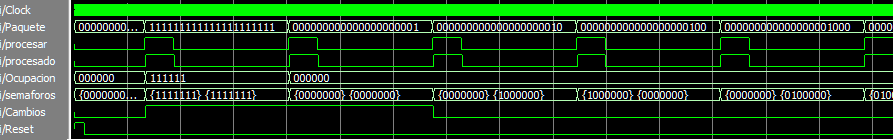
\includegraphics[scale=0.6]{./Figures/Test/Separador}
			\caption{Simulación del separador}
			\label{fig:Test_Separador}
		\end{figure}
		
		Figura \ref{fig:Test_Enclavamiento} ...
		
		\begin{figure}[h]
		\centering
		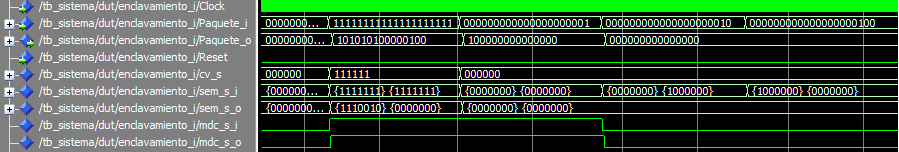
\includegraphics[scale=0.65]{./Figures/Test/Enclavamiento}
			\caption{Simulación del enclavamiento}
			\label{fig:Test_Enclavamiento}
		\end{figure}
		
		Figura \ref{fig:Test_Mediador} ...
		
		\begin{figure}[h]
		\centering
		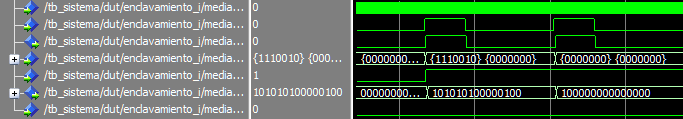
\includegraphics[scale=0.8]{./Figures/Test/Mediador}
			\caption{Simulación del mediador}
			\label{fig:Test_Mediador}
		\end{figure}
		

\section{Validación del registro}

	\subsection{Testbench del módulo registro}
			
		Se generó el Algoritmo \ref{lst:test_registro} para ...
		
			
		\begin{lstlisting}[language = vhdl,caption=Testbench del módulo registro,label={lst:test_registro}] 
				
			library ieee;
use ieee.std_logic_1164.all;

entity tb_registro is
end tb_registro;

architecture tb of tb_registro is

    component registro is
	port(
		clk_i: in std_logic;
        	rst_i: in std_logic;
 	        paquete_ok : in std_logic;
  	        paquete_i: in std_logic_vector(15-1 downto 0);
  	        w_data: out std_logic_vector(8-1 downto 0);
  	        wr_uart : out std_logic  -- "char_disp"
	);
    end component;

    signal clk_i     : std_logic;
    signal rst_i     : std_logic;
    signal paquete_ok     : std_logic;
    signal paquete_i   : std_logic_vector (15-1 downto 0); 
    signal w_data    : std_logic_vector (8-1 downto 0);
    signal wr_uart : std_logic;

    constant TbPeriod : time := 8 ns; -- EDIT Put right period here
    signal TbClock : std_logic := '0';
    signal TbSimEnded : std_logic := '0';

begin

    dut : registro
    port map (clk_i      => clk_i,
              rst_i      => rst_i,
              paquete_i   => paquete_i,
              paquete_ok => paquete_ok,
              w_data     => w_data,
 	      wr_uart    => wr_uart);

    -- Clock generation
    TbClock <= not TbClock after TbPeriod/2 when TbSimEnded /= '1' else '0';

    -- EDIT: Check that clk_i is really your main clock signal
    clk_i <= TbClock;

    
	
    stimuli : process
    begin
        -- EDIT Adapt initialization as needed
        --r_data <= (others => '0');

        -- Reset generation
        -- EDIT: Check that rst_i is really your reset signal
        rst_i <= '1';
        wait for 20 ns;
        rst_i <= '0';
	wait for 1 ns;
	
        wait for 1000000 * TbPeriod;

        -- Stop the clock and hence terminate the simulation
        --TbSimEnded <= '1';
        --wait;
    end process;

    datos : process
    begin
        
        
        paquete_i <= "101010101010101";
	paquete_ok <= '1';
 	wait for 1000 * TbPeriod;
	paquete_ok <= '0';
	
	wait for 1000 * TbPeriod;

	paquete_i <= "110110110110110";
 	paquete_ok <= '1';
 	wait for 1000 * TbPeriod;
	paquete_ok <= '0';

	

        --wait for 100 * TbPeriod;
	--TbSimEnded <= '1';
    end process;
	
end tb;
		\end{lstlisting}
			
	\subsection{Resultados obtenidos}
				
		Figura \ref{fig:Test_Registro} ...
		
	\begin{figure}[h]
	\centering
	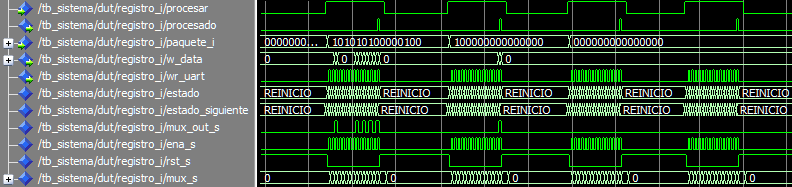
\includegraphics[scale=0.7]{./Figures/Test/Registro}
		\caption{Simulación del registro}
		\label{fig:Test_Registro}
	\end{figure}
	
\section{Validación del selector}

	\subsection{Testbench del módulo selector}
			
		Se generó el Algoritmo \ref{lst:test_selector} para ...
		
			
		\begin{lstlisting}[language = vhdl,caption=Testbench del módulo selector,label={lst:test_selector}] 
				
			library ieee;
use ieee.std_logic_1164.all;

entity tb_conector_test is
end tb_conector_test;

architecture tb of tb_conector_test is

    component conector_test
        port(
		clk_i: in std_logic;
        	rst_i: in std_logic;
        	switch : in std_logic;
        	leds : out std_logic_vector(2-1 downto 0);
        	wr_uart_3 : out std_logic;
       	 	N_1 : in integer;
       	 	N_2 : in integer;
        	r_disponible : in std_logic;
        	w_data_1: in std_logic_vector(8-1 downto 0);
        	w_data_2: in std_logic_vector(8-1 downto 0);
        	w_data_3: out std_logic_vector(8-1 downto 0)
	);
    end component;

    signal clk_i,rst_i,switch,wr_uart_3,r_disponible     : std_logic;
    signal leds      : std_logic_vector(2-1 downto 0);
    signal N_1,N_2   : integer;
    signal w_data_1,w_data_2,w_data_3 : std_logic_vector(8-1 downto 0);

    constant TbPeriod : time := 8 ns; -- EDIT Put right period here
    signal TbClock : std_logic := '0';
    signal TbSimEnded : std_logic := '0';

	 -- Low-level byte-write
  	procedure Enviar_char (
    		data       : in  std_logic_vector(8-1 downto 0);
    		signal r_data : out std_logic_vector(8-1 downto 0);
		signal r_disponible : out std_logic) is
  	begin
		
		r_disponible <= '0';
		wait for TbPeriod;
        	r_data <= data;
		wait for 407 * TbPeriod;
		r_disponible <= '1';
		wait for TbPeriod;
		r_disponible <= '0';

  	end Enviar_char;

begin

    dut : conector_test
    port map (clk_i      => clk_i,
              rst_i      => rst_i,
              switch     => switch,
	      leds 	 => leds,
              wr_uart_3  => wr_uart_3,
              N_1  	 => N_1,
              N_2    	 => N_2,
	      r_disponible => r_disponible,
	      w_data_1   => w_data_1,
	      w_data_2   => w_data_2,
	      w_data_3   => w_data_3);
 
    -- Clock generation
    TbClock <= not TbClock after TbPeriod/2 when TbSimEnded /= '1' else '0';

    -- EDIT: Check that clk_i is really your main clock signal
    clk_i <= TbClock;

    stimuli : process
    begin
        -- EDIT Adapt initialization as needed
        --r_data <= (others => '0');

        -- Reset generation
        -- EDIT: Check that rst_i is really your reset signal
        rst_i <= '1';
        wait for 100 ns;
        rst_i <= '0';

	
        wait for 1000000 * TbPeriod;

        -- Stop the clock and hence terminate the simulation
        TbSimEnded <= '1';
        wait;
    end process;

    datos : process
    begin
        
	w_data_2 <= "00000000";
	N_2 <= 0;
	switch <= '0';

	wait for 200 ns;

	-- 21
	N_1 <= 23; 	
	r_disponible <= '1';
	--wait for 5 * TbPeriod;
	Enviar_char("00111100",w_data_1,r_disponible); -- < 	
	Enviar_char("00110001",w_data_1,r_disponible); -- 1 	
	Enviar_char("00110001",w_data_1,r_disponible); -- 1
 	Enviar_char("00110001",w_data_1,r_disponible); -- 1 	
	Enviar_char("00110000",w_data_1,r_disponible); -- 0
	Enviar_char("00110001",w_data_1,r_disponible); -- 1 	
	Enviar_char("00110000",w_data_1,r_disponible); -- 0
	Enviar_char("00110001",w_data_1,r_disponible); -- 1 	
	Enviar_char("00110000",w_data_1,r_disponible); -- 0
	Enviar_char("00110001",w_data_1,r_disponible); -- 1 	
	Enviar_char("00110000",w_data_1,r_disponible); -- 0
	Enviar_char("00110001",w_data_1,r_disponible); -- 1 	
	Enviar_char("00110000",w_data_1,r_disponible); -- 0
	Enviar_char("00110001",w_data_1,r_disponible); -- 1 	
	Enviar_char("00110000",w_data_1,r_disponible); -- 0
	Enviar_char("00110001",w_data_1,r_disponible); -- 1 	
	Enviar_char("00110000",w_data_1,r_disponible); -- 0
	Enviar_char("00110001",w_data_1,r_disponible); -- 1 	
	Enviar_char("00110000",w_data_1,r_disponible); -- 0
	Enviar_char("00110000",w_data_1,r_disponible); -- 0	
	Enviar_char("00110001",w_data_1,r_disponible); -- 1 
	Enviar_char("00110001",w_data_1,r_disponible); -- 1 	
	Enviar_char("00111110",w_data_1,r_disponible); -- >
	--wait for 5 * TbPeriod;
	r_disponible <= '0';
	wait for 1000 * TbPeriod;

        --wait for 100 * TbPeriod;
	--TbSimEnded <= '1';
    end process;
	
end tb;
		\end{lstlisting}
			
	\subsection{Resultados obtenidos}
				
		Figura \ref{fig:Test_Selector} ...
		
	\begin{figure}[h]
	\centering
	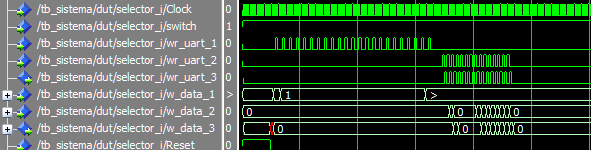
\includegraphics[scale=0.95]{./Figures/Test/Selector}
		\caption{Simulación del selector}
		\label{fig:Test_Selector}
	\end{figure}
			